\clearpage
\section{Design and Implementation}

At this point the project has a set of requirements to meet and basic solution approach has been outlined for each aspect of 
the project.
This section aims to inform the reader of the detailed design choices made and how this was implemented to achieve the final product.

\subsection{System model design} \label{system model design}

\begin{figure}[ht]
    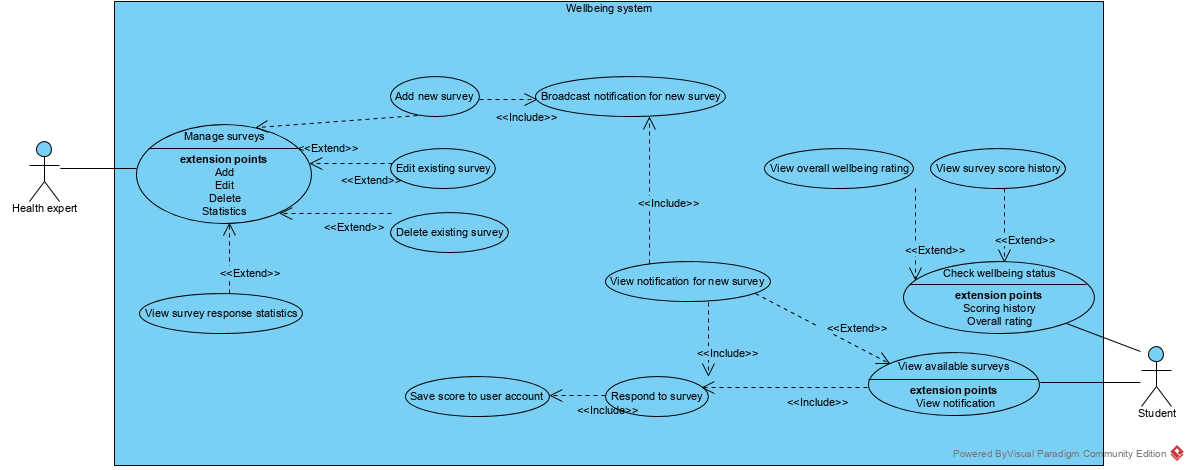
\includegraphics[width=450px]{images/system_model.png}
    \caption{Proposed system model}
\end{figure}


The proposed system model outlines the method in which an \textit{expert} can create, edit or delete a survey and how this can be 
fed to a student.
The main functionality to point out, that really links the two user types together, is how new survey send some sort notification 
to a (potentially) subscribed student; leading them to respond to the survey.
From the diagram, the reader should be able to see how a student will be able to either view surveys at their own will or be prompted
by a notification that had been sent out by some service.
The system outlines that there are really only two different categories of user that will use the system, this makes sense when looking
back at the articulation of the problem and the original brief given.

\clearpage
\subsection{Flow diagram}

An important process for the software solution is to be able to add and modify surveys for students to respond to.
The system model design does not go into much detail about this part of the system so it will be important to gain some clarity around this area.
Below is the proposed process flow diagram for what will occur when a user, of the system, attempts to add a new survey.
It outlines the need for authorisation (have permission to access such a resource) before carrying out two steps of validation of the
data provided.
If validation passes, then the survey and survey questions entries will be added to the database.
As mentioned in the system model design, there is a mention of the notification service that will alert students about a new survey they
can participate in.
The flow diagram shows how an expert can be prompted about sending out an alert to students, after submitting the survey.
That is where the system will then move onto executing the notification service, or just conclude the current process flow.

\begin{figure}[ht]
    \centering
    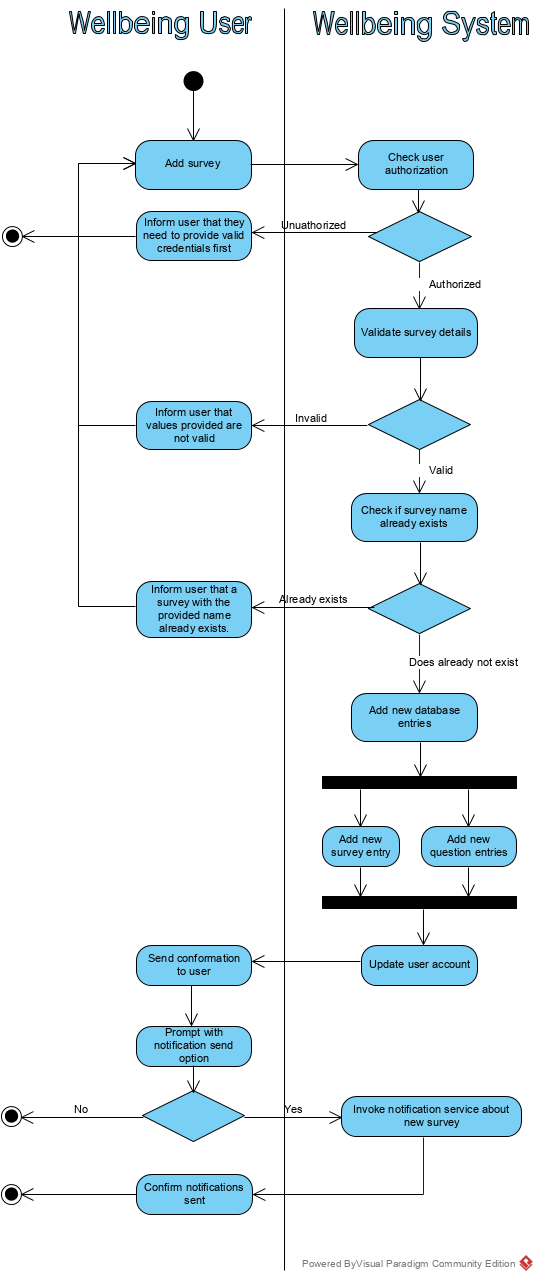
\includegraphics[width=150px]{images/flow_diagram.png}
    \caption{Flow diagram of the processes involved when an \textit{expert} adds a new survey}
\end{figure}

\clearpage

\subsection{Database (data layer)}
The database is important to get right as the design needs to store surveys data in a logical structured manner.
To understand what is required for the database, it makes sense to first break it down and understand relationships between
each entity.

\begin{enumerate}
    \item Each \textit{survey} will have a survey name or title and has a \textit{one-to-many} relationship with \textit{survey questions}.
    \item Each \textit{survey question} will have a question name and will have a \textit{one-to-many} relationship with \textit{question choices}.
    \item Each \textit{question choice} will have a choice name with an associated weight.
    \item To store user choices for a \textit{survey question} a \textit{user question choice} entity can be used.
        \begin{enumerate}
            \item Each \textit{user question choice} will have a \textit{many-to-one} relationship with a \textit{survey question} and \textit{question choice}
        \end{enumerate}
\end{enumerate}

To map out these relationships, into a diagram that can be visually understood, JDL (JHipster Domain Language) was used.
The JDL approach allows for a more logical approach of designing a database since it avoids any confusion from a purely visual approach.
Below is the JDL written with the associated diagram representation.

\begin{figure}[ht]
    \centering
    \begin{lstlisting}[language=JDL]
entity UserQuestionChoice {
	timeStamp Timestamp
}
entity Choice {
	choice String,
    weight Integer
}
entity Question {
	question String
}
entity Survey {
	description String
}
relationship OneToMany {
    Survey{survey} to Question{survey}
	Question{question} to Choice
}
relationship ManyToOne {
    UserQuestionChoice to Question
    UserQuestionChoice to Choice
}
    \end{lstlisting}
    \caption{JDL based on the breakdown of what will be needed to store surveys}
\end{figure}

\clearpage
\begin{figure}[ht]
    \centering
    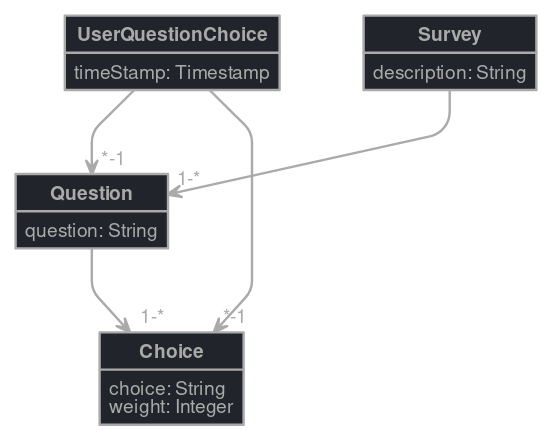
\includegraphics[width=250px]{images/jhipster-jdl.png}
    \caption{Graph produced by JDL-studio}
    \label{survey-jdl-graph}
\end{figure}

Since initial prototyping is being done using the JHipster framework, it makes sense to take advantage of tools such as 
JDL-studio to produce diagrams such as \ref{survey-jdl-graph}.
To fully take advantage of the JDL written, it can be imported into the JHipster product being worked on. 
The functionality of value that will be desired from the import process will be a set of generated classes that represent
the database schema.

\subsubsection{Java Persistence API}
An SQL database schema can be created in Java itself with the help of Hibernate. % You might want to go over this in the lit review.
Hibernate will facilitate the mapping of object-orientated domains, created in Java, to the corresponding tables in a relational database.
The Java Persistence API (JPA) set of packages will provide the necessary annotations to correctly set up classes that represent \textit{tables}.
Figure \ref{question object} shows how a class, with all the required annotations, can be created.
Domain classes that are created, as a part of the Java code, use the Java Persistence API (JPA) set of packages.
The JPA packages provide the required annotations to be used in a class to allow a chosen mapping tool (Hibernate in this case) to understand how
to map class objects into database tables.
Cascading options are also available to allow actions on an entry in the table to be reflected on any child entities.
In the example below, cascading is used to ensure that if a \textit{question} is removed from the database, any \textit{question choices} associated
with it are also removed; ensuring no orphan entries are produced in the database.

\clearpage
\begin{figure}[ht]
    \centering
    \begin{lstlisting}[language=Java]
@Entity
@Table(name = "question")
public class Question implements Serializable {
    private static final long serialVersionUID = 1L;
    @Id
    @GeneratedValue(strategy = GenerationType.IDENTITY)
    private Long id;
    @Column(name = "question")
    private String question;
    @OneToMany(mappedBy = "question", cascade = CascadeType.ALL)
    @JsonProperty(access = JsonProperty.Access.READ_ONLY)
    private Set<Choice> questionChoices = new HashSet<>();
    @ManyToOne(fetch = FetchType.EAGER, optional = false)
    @JoinColumn(name = "survey_id", nullable = false)
    @JsonIgnore
    private Survey survey;
    @OneToMany(mappedBy = "question", cascade = CascadeType.ALL)
    private Set<UserQuestionChoice> userQuestionChoices = new HashSet<>();
    \end{lstlisting}
    \caption{Question object to be mapped to a database table}
    \label{question object}
\end{figure}


The benefit of this approach is that the database schema can be controlled programatically and also allows for repository interfaces to be created.
Repository interfaces is what is used to invoke actions against the corresponding table in the database.
A notable feature of these interfaces is that they allow for \textit{derived} methods to be written without having to write any logic for it.
The idea behind these derived methods is that it gives flexibility to the developer to incorporate query methods to a specific problem.
It is also important to note that there is no SQL being written as a part of the code; only Java code is being written.


\begin{figure}[ht]
    \centering
    \begin{lstlisting}[language=Java]
@Repository
public interface QuestionRepository extends JpaRepository<Question,Long> 
{
    List<Question> findBySurveyId(Long surveyId);
    Optional<Question> findByIdAndSurveyId(Long id, Long surveyId);
    boolean existsByIdAndSurveyId(Long id, Long surveyId);

    @Transactional
    @Modifying
    void deleteByIdAndSurveyId(Long id, Long surveyId);
}
    \end{lstlisting}
    \caption{Repository interface for Question domain/table}
    \label{repo example}
\end{figure}


Now that the main Java components have been covered, Spring will need to be configured to actually connect to a database.
For this project, a MySQL container will be configured. To do this, a \textit{docker compose} file can be created.
As shown in figure \ref{sqldocker}, the file allows for environment variables and exposed ports to be specified.
Once the file is ready, the command \textit{docker-compose up compose.yml} can be run.
This command will pull down the docker image and automatically start it along with applying the specified options in the file.
After logs start appearing in the command-line, a connection attempt to the database can be made using a tool such as MySQLWorkbench.
Using a tool such as MySQLWorkbench is important as it allows for manual SQL queries to be run against the database and verify that operations
executed by hibernate are doing the right thing.


\begin{figure}[ht]
    \centering
    \begin{lstlisting}
#compose version of 3.3        
version: '3.3'
services:
  db:
    image: mysql
    restart: always
    environment:
      MYSQL_DATABASE: 'springdb'
      MYSQL_USER: 'admin'
      MYSQL_PASSWORD: 'admin'
      MYSQL_ROOT_PASSWORD: 'password'
      lower_case_table_names: '1'
      character_set_server: 'utf8'
    ports:
      # <Port exposed> : < MySQL Port running inside container>
      - '3306:3306'
    expose:
      # Opens port 3306 on the container
      - '3306'           
    \end{lstlisting}
    \caption{Docker compose yaml file for a mysql image from dockerhub}
    \label{sqldocker}
\end{figure}

Spring still needs to be configured to actually connect to this database running in a container.
The details required will be the database name with valid login credentials.
An application.yml (yaml file) is used by spring to configure various aspects of the project, depending on what is required by the developer.
Below, in figure \ref{springymldbconfig}, the reader can see the simple configuration needed to get a database connection set up.
The SpringBoot application will automatically read and apply the configuration on the initial start up; if anything is wrong with the config,
and exception will be thrown and stop the server.

\begin{figure}[ht]
    \centering
    \begin{lstlisting}[escapechar=|]
spring:
    datasource:
        url: jdbc:mysql://localhost:3306/springdb
        driver-class-name: com.mysql.cj.jdbc.Driver
        username: root
        password: password
    jpa:
        database: mysql
        show-sql: true
        hibernate:
            ddl-auto: update |\label{hibernate option}|
    \end{lstlisting}
    \caption{Snippet from application.yml for configuring the spring project}
    \label{springymldbconfig}
\end{figure}

\clearpage
\subsubsection{Final DB schema}

\begin{figure}[ht]
    \centering
    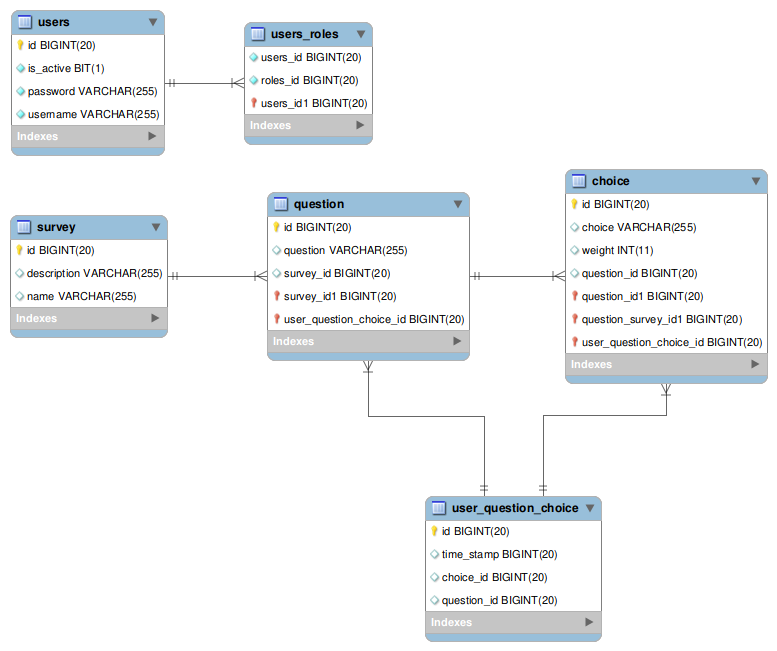
\includegraphics[width=300px]{images/db_schema.png}
    \caption{Database schema diagram produced from MySQLWorkbench}
    \label{sqldbschamfull}
\end{figure}

Once everything has been correctly configured, the SpringBoot application can be run.
Line \ref{hibernate option}, in figure \ref{springymldbconfig} be set to either \textit{create} or \textit{update}.
The main difference between the two is that \textit{create} will always overwrite any existing schema whereas \textit{update} will not.



\subsection{REST API}
% Talk about how it is going to be used
% Outline the main endpoints that need to be implemented
% Detail the endpoints that have been implemented and what they do

The REST API, to be implemented, is going to be a very important part of this project as it will be means of communicating between
the server and client. 
As mentioned in section \ref{restliterature}, a set of URL based endpoints will need to be defined as a part of the API 
documentation.
The URL paths themselves will be based on the type of access needed to resources of the system, most notably survey and user data.
Since this is an application that focuses on creating and responding to surveys, the API defined will have to focus on that.
The REST endpoints will be based on the system model diagram in section \ref{system model design} as it outlines the use cases 
of the system.
Designing the API will heavily revolve around the database schema as shown in figure \ref{sqldbschamfull}.


% I think here i would want to get tables written with explanations of the api
% After the tables are written, then talk about how it's implemented with code snippets of Controller classes.



\subsection{Spring security}

Talk about spring security aspects that you have implemented
oauth2 and jwt are good examples
what else?



\subsection{REACT client}
Talk about everything to do with the implementation of the REST client
State how you started off from that OKTA example and worked from there. 
